\documentclass[a4paper,12pt]{article}

%% Language and font encodings
\usepackage[english]{babel}
\usepackage[utf8]{inputenc}
\usepackage[T1]{fontenc}


%% Sets page size and margins
\usepackage[a4paper,top=3cm,bottom=3cm,left=2cm,right=2cm]{geometry}

\usepackage[colorlinks,urlcolor=blue,linkcolor=blue,citecolor=blue]{hyperref}

%% Useful packages
%%%% TikZ %%%%
\usepackage{tikz}
\usetikzlibrary{shapes,fit,positioning,arrows,decorations.markings}

%% Fancy layout
\usepackage{fancyhdr}
\pagestyle{fancy}
\fancyhead[L]{}
\fancyhead[C]{
\includegraphics[scale=0.2]{logo.jpg}}
\fancyhead[R]{R. Detobel}
% Footer
\fancyfoot[C]{}
\fancyfoot[R]{page \thepage}
% Line
\renewcommand{\headrulewidth}{0.4pt}
\renewcommand{\footrulewidth}{0.4pt}

\let\oldemph\emph
\renewcommand{\emph}[1]{\textbf{\oldemph{#1}}}

\setlength{\headheight}{20pt}

%opening
\title{INFO-F-530: Computer Science Seminar}
\author{Rémy Detobel}

\setlength{\parindent}{0cm}

\begin{document}

%%%%%%%%%%%%%%%%
\begin{titlepage}
\begin{center}
\textbf{UNIVERSIT\'E LIBRE DE BRUXELLES}\\
\textbf{Faculté des Sciences}\\
\textbf{Département d'Informatique}
\vfill{}\vfill{}

%\begin{center}
{\Huge  Traitement d'un flux de données \vspace*{.5cm}  \linebreak[4] spatio-temporel avec PostgreSQL}
%\end{center}

{\Huge \par \vspace*{1cm}}
\begin{center}{\LARGE \textbf{Post documentation:} Install solution}\end{center}{\Huge \par}

{\Huge \par}
\begin{center}{\LARGE Rémy Detobel}\end{center}{\Huge \par}
\vfill{}\vfill{}
\begin{flushright}{\large \textbf{Promoteur :}}\\
{\large Prof. Esteban Zimanyi}\end{flushright}{\large\par}
\vfill{}\vfill{}\enlargethispage{3cm}
\textbf{Année académique 2018~-~2019}
\end{center}
\end{titlepage}
\newpage

\tableofcontents
\newpage

\section{Introduction}

    \subsection{Français}
        Ce document est une documentation complémentaire au mémoire ``Traitement d'un flux de données spatio-temporel avec PostgreSQL''. Le travail lié à ce mémoire a nécéssité plusieurs tests et divers mises en places.\\
        
        Ce document vise donc à expliquer les différentes structures crées et leurs mises en place. Tous les codes ont été regroupé sur un repos Github: \url{https://github.com/detobel36/MobilityDBComparison}\\
        Pour des raisons de facilité, ce document sera écrit en anglais. Notez que le mémoire est lui en français.
        
        
    \subsection{English}
        This document is a complementary documentation for the master thesis ``Traitement d'un flux de données spatio-temporel avec PostgreSQL''. The work linked to this master thesis required multiple tests and various set up.\\
        
        This document try to explain the different architecture and how to set up them. All code has been push on a Github repository: \url{https://github.com/detobel36/MobilityDBComparison}\\
        For easy of use, this document has been writen in English. Notice that the master thesis is in french.

        
\section{Architecture}
    In this section we will see the existing structure but also the architecture that could be set up.
    
    \subsection{Servers}
        The project has evolved in time. At the beginning a server (from ULB) was used to try some solutions: ``Tristan23''. But after several tests, it seems that Barefoot was consuming a lot of memory. Thus, tests were set up on this first server (``Tristan23'') and ``production'' was set up on another server: ``GeoData''.\\
        
        These two servers are managed by the ULB and for security reason they aren't accessible with web protocol (without a complicated authentification set up). So to display easily results, a new server was used. This new server is a private server (rent by ``R. Detobel'').\\
        
        To summarize, in this project, three servers were used:
        \begin{itemize}
            \item GeoData: for production;
            \item Tristan23: for testing;
            \item Private: for web server.
        \end{itemize}
        
    \subsection{Existing architecture}
        \label{subsec:exist_architecture}
        The image \ref{img:exist_architecture} show the end architecutre set up.
        \begin{figure}[h]
            \centering
            \begin{tikzpicture}
                % --------
                % GeoData
                % --------
                \node[draw, align=center] at (0, 0) (source) {Data source\\MTA};
                
                \node[draw, align=center] at (3, 0) (script) {Script};
                
                \node[draw, align=center] at (7, 1) (socket) {Socket};
                \node[draw, align=center] at (6, -1) (archive) {Archives};
                
                \node[draw, align=center] at (8, -1) (script2) {Script};
                \node[draw, align=center] at (12, 0) (barefoot) {MTA Barefoot};
                
                \node[draw, align=center] at (4.5, -3) (pipelinedb) {PipelineDB};
                \node[draw, align=center] at (7.5, -3) (postgresql) {PostgreSQL};
                \node[draw, align=center] at (6, -4) (timescaledb) {TimescaleDB};
                
                \node[draw,fit=(postgresql) (pipelinedb) (timescaledb)] (db) {};
                \node (textDb) at (db.north) [above] {Database};
                
                % Draw line
                \draw[->,thick,shorten <=2pt,shorten >=4pt,>=stealth] (source) -- (script);
                \draw[->,thick,shorten <=2pt,shorten >=4pt,>=stealth] (script) -- (socket);
                \draw[->,thick,shorten <=2pt,shorten >=4pt,>=stealth] (script) -- (archive);
                \draw[<-,thick,shorten <=2pt,shorten >=4pt,>=stealth] (archive) -- (script2);
                \draw[<-,thick,shorten <=2pt,shorten >=4pt,>=stealth] (socket) -- (barefoot);
                \draw[->,thick,shorten <=2pt,shorten >=4pt,>=stealth] (script2) -- (barefoot);
                \draw[->,thick,shorten <=2pt,shorten >=4pt,>=stealth] (barefoot) -- (db.east);
                
                % Create GeoData
                \node[draw,fit=(source) (script) (socket) (archive) (script2) (barefoot) (db) (textDb)] (geodata) {};
                \node (textGeodata) at (geodata.north) [above] {GeoData};
                
                
                % --------
                % Private
                % --------
                \node[draw, align=center] at (6.5, -7) (pipelinedb2) {PipelineDB};
                \node[draw, align=center] at (9.5, -7) (postgresql2) {PostgreSQL};
                \node[draw, align=center] at (8, -8) (timescaledb2) {TimescaleDB};
                
                \node[draw,fit=(postgresql2) (pipelinedb2) (timescaledb2)] (db2) {};
                \node (textDb2) at (db2.north) [above] {Database};
                
                \node[draw, align=center] at (2, -7.5) (webserver) {Web Server};
                
                % Draw line
                \draw[->,thick,shorten <=2pt,shorten >=4pt,>=stealth] (barefoot) -- (db2.east);
                \draw[->,thick,shorten <=2pt,shorten >=4pt,>=stealth] (webserver) -- (db2);
                
                % Create private
                \node[draw,fit=(webserver) (db2) (textDb2)] (private) {};
                \node (textPrivate) at (private.north) [above] {Private};
                
            \end{tikzpicture}
            \caption{Existing architecture}
            \label{img:exist_architecture}
        \end{figure}
        This architecture make computation on GeoData server and results are displayed on private serveur. Notice that we need to choose: store the result on GeoData (to mesure performance) or store result on private server to display results.\\
        
        The ``Tristan23'' server isn't displayed in this image because it is only used to set up new solution and test that they work.
        
        
    \subsection{Possible architecture}
        The section \ref{subsec:exist_architecture} present the current solution, which respect some hardware constraint (server access, performances...).\\
        
        The solution present by the figure \ref{img:exist_architecture} could be simplified to have only one server. It is this solution that is presented in the image \ref{img:new_architecture}.
        \begin{figure}[h]
            \centering
            \begin{tikzpicture}
                % --------
                % GeoData
                % --------
                \node[draw, align=center] at (0, 0) (source) {Data source\\MTA};
                
                \node[draw, align=center] at (3, 0) (script) {Script};
                
                \node[draw, align=center] at (7, 1) (socket) {Socket};
                \node[draw, align=center] at (6, -1) (archive) {Archives};
                
                \node[draw, align=center] at (8, -1) (script2) {Script};
                \node[draw, align=center] at (12, 0) (barefoot) {MTA Barefoot};
                
                \node[draw, align=center] at (4.5, -3) (pipelinedb) {PipelineDB};
                \node[draw, align=center] at (7.5, -3) (postgresql) {PostgreSQL};
                \node[draw, align=center] at (6, -4) (timescaledb) {TimescaleDB};
                
                \node[draw,fit=(postgresql) (pipelinedb) (timescaledb)] (db) {};
                \node (textDb) at (db.north) [above] {Database};
                
                \node[draw, align=center] at (0.5, -3.5) (webserver) {Web Server};
                
                % Draw line
                \draw[->,thick,shorten <=2pt,shorten >=4pt,>=stealth] (source) -- (script);
                \draw[->,thick,shorten <=2pt,shorten >=4pt,>=stealth] (script) -- (socket);
                \draw[->,thick,shorten <=2pt,shorten >=4pt,>=stealth] (script) -- (archive);
                \draw[<-,thick,shorten <=2pt,shorten >=4pt,>=stealth] (archive) -- (script2);
                \draw[<-,thick,shorten <=2pt,shorten >=4pt,>=stealth] (socket) -- (barefoot);
                \draw[->,thick,shorten <=2pt,shorten >=4pt,>=stealth] (script2) -- (barefoot);
                \draw[->,thick,shorten <=2pt,shorten >=4pt,>=stealth] (barefoot) -- (db.east);                
                
                \draw[->,thick,shorten <=2pt,shorten >=4pt,>=stealth] (webserver) -- (db);
            \end{tikzpicture}
            \caption{Possible architecture}
            \label{img:new_architecture}
        \end{figure}
        The different programs used in this image will be detailed in the following points. Note that they must not all be on the same server. Most of the connections made between the different programs can be adapted to a remote solution (socket, SQL query, file recovery (especially archives)...).
        
        
\section{Programs and configuration}
    This section will describe programs mentioned before. The goal is to explain the differents step to set up and configure these programs.
    
    \subsection{Script to fetch data source}
        \label{subsec:script_fetch_data}
        In the figure \ref{img:exist_architecture} and \ref{img:new_architecture}, first elements are: ``Data source MTA'', ``Script'' (twice) and ``Archives''. These elements are set up by ULB.\\
        This document will not details how it work but, to summarize it is simply a GET query send to MTA server which fetch information and create a stream socket in addition to store the content of the result into a file.
    
    \subsection{MTA Barefoot}
        ``MTA Barefoot'' is a modified version of Barefoot. In fact it is more of a Java program using Barefoot as a library. The goal is to allow different methods to send information into Barefoot.\\
        
        \subsubsection{Build}
            The code of ``MTA Barefoot'' is accessible here: \url{https://github.com/detobel36/MTABarefoot}\\
            To get the executable file (with the extension ``.jar''), you only need to execute the following command: \verb|mvn clean build|
            
            You will get a folder ``target'' with two executables. One of them directly includes the Barefoot library (the one containing, logically, "with-dependencies" in its name).
        
        \subsubsection{Start}
            To start the executable you can execute the following command: 
            \begin{verbatim}
java -jar <jar file> </path/to/server/properties> </path/to/mapserver/properties>
    [INPUT: server/mta/socket] [OUTPUT: tcp/sql]\end{verbatim}
            The first parameter is the name of the executable. The second and the third parameters define some configuration file. The two following parameters define which method must be used to (respectively) get input information and push output information.\\
            
            For the configuration, the second argument reference the server configuration. ``MTA Barefoot'' is based on ``Track server'' (from Barefoot). The same configuration could be used. An example is available here: \url{https://github.com/detobel36/MobilityDBComparison/tree/master/Tool/config}\\
            
            For the third parameters, it is information to connect to database. An example of configuration could be find here: \url{https://github.com/detobel36/MobilityDBComparison/blob/master/Tool/config/map_server.properties}\\
            Notice that in image \ref{img:exist_architecture} the database could be on localhost or in remove. To switch easily between these two configuration, the script \verb|switchConfig.sh| was used (available \href{https://github.com/detobel36/MobilityDBComparison/blob/master/Tool/switchConfig.sh}{here}).\\
            
            There are three different type of input for ``MTA Barefoot'':
            \begin{itemize}
                \item ``server'' to have a listen port socket (define in server configuration);
                \item ``mta'' which will fetch directly information on MTA server;
                \item ``socket'' which will listen to ``local'' socket, define by the script (define in point \ref{subsec:script_fetch_data}).
            \end{itemize}
            
            For the output solution, two method are available: tcp and sql. The first one come from original code of Barefoot. The goal is to have a server (NodeJS) which lisen to a TCP connection and directly display result (on web). In this configuration nothing is done to save data.\\
            The ``SQL'' output allow to execute one or multiple SQL Query when a position is treat. Queries which must be executed are store in the file \verb|request.sql|, present in the ``config`` folder. You will find an example \href{https://github.com/detobel36/MobilityDBComparison/blob/master/Tool/config/request.sql}{here}. MTA Barefoot will automaticaly detect if there is one or multiple query (based on '';`` symbol).\\
            Variable could be used in queries. The variable have the following syntax: ''\verb|:name |''. Notice the space after the variable name.\\
            
            Possible variables in queries process by Barefoot:
            \begin{itemize}
                \item \verb|:trip_id | (given by MTA API);
                \item \verb|:start_date | (given by MTA API (type: integer));
                \item \verb|:route_id | (given by MTA API);
                \item \verb|:direction_id | (given by MTA API);
                \item \verb|:bearing | (given by MTA API);
                \item \verb|:stop_id | (given by MTA API);
                \item \verb|:time | (time of the point);
                \item \verb|:point | (encode as \verb|POINT(x, y)|);
                \item \verb|:route | (sequence of point that compose road);
                \item \verb|:candidates | (JSON with candidate point (never test on SQL query));
                \item \verb|:distance | (distance between last and current point);
                \item \verb|:timeDiff | (difference in time between last and current point);
                \item \verb|:speed | (speed average in km/h between last and current point (based on two last information));
                \item \verb|:timeRoad | (contain all ``road'' point (and information) between last and current point (never test on SQL query));
                \item \verb|:timeCoordinate | (contain all point (on the road) between last and current point with the MobilityDB format).
            \end{itemize}

    \subsection{Database}
        The database is a PostgreSQL database with different extensions. Install instruction of extensions are available directly on respective documentation:
        \begin{itemize}
            \item MobilityDB, more information here: \url{https://github.com/ULB-CoDE-WIT/MobilityDB}
            \item PipelineDB, more information here: \url{http://docs.pipelinedb.com/installation.html#install-postgresql}
            \item TimescaleDB, more information here: \url{https://docs.timescale.com/v1.3/getting-started/installation}
        \end{itemize}
        In this project differents solutions have been tested. Tables are not the same for each solution. But to test these solutions, some other data (and thus tables) are required.
        \begin{itemize}
            \item \verb|usa_adm| which contains counties of USA.\\
                The script \verb|import.sh| in the folder \href{https://github.com/detobel36/MobilityDBComparison/tree/master/Tool/NewYorkCounty}{NewYorkCounty} could be used to create the table and import the data.
            \item \verb|gtfs_shape_geoms| which contains bus road of New York.\\
                The folder ``Tool'' contain a script to create and import easily the data. \url{https://github.com/detobel36/MobilityDBComparison/blob/master/Tool/importGtfsMta.sh}
        \end{itemize}
        
        As already mentioned, the database is based on PostgreSQL. Extensions are then added to improve or add elements to the database. Each extension allows you to create a new solution. For some solutions, variants can also be tested. Concretely, there are 5 choices:
        \begin{itemize}
            \item PostgreSQL with pre-treatment;
            \item PostgreSQL with post-treatment;
            \item PipelineDB;
            \item TimescaleDB with pre-treatment;
            \item TimescaleDB with post-treatment.
        \end{itemize}
        For each solution, 3 files have been created in the folder \href{https://github.com/detobel36/MobilityDBComparison/tree/master/Script}{Script}: one for the initialisation, one for the insert query and the last for the selection.\\
        
        The setup of a solution is describe in the point \ref{sec:link_technologies}.
        
        
    \subsection{Website}
        \label{sec:webiste}
        To set up a website to view result you just need to install a web server (the current solution have been test with Apache2) and install PHP 7.0 (or upper).\\
        
        Then you need to add \href{https://github.com/detobel36/MobilityDBComparison/tree/master/Website}{following folder} in your ``web home'' folder.\\
        
        A small configuration is needed:
        \begin{itemize}
            \item For database, you need to update the file \verb|model/bdd.php| with your own PostgreSQL configuration.
            \item For webiste parameter, you need to update the file \verb|controllers/useful.php|, where you need to update Google Key and Website URL.
        \end{itemize}
        
        All files in this website are not up-to-date. The interesing pages have the prefix \verb|visual|. For instance ``visualDashboard'' (the URL will be \verb|http://your_website.com/visualDashboard|) allow you to see the first case develop in the ``Result'' section of the master Thesis.\\
        
        In the master thesis, 3 cases were studied: bus informations, bus deviation and time in county (also named ``zone''). Each case have two files: one to made the SQL query and another to display result. Notice that a Javascript code is also define for each case (check the folder \href{https://github.com/detobel36/MobilityDBComparison/tree/master/Website/assets/js}{assets/js}.
        \begin{itemize}
            \item \textbf{Bus information:}\\
                The SQL query is in the file \href{https://github.com/detobel36/MobilityDBComparison/blob/master/Website/controllers/getVisualDashboardData.php}{getVisualDashboardData.php}\\
                The display page is the file \href{https://github.com/detobel36/MobilityDBComparison/blob/master/Website/controllers/visualDashboard.php}{visualDashboard.php}
            \item \textbf{Bus deviation:}\\
                SQL Query: \href{https://github.com/detobel36/MobilityDBComparison/blob/master/Website/controllers/getDeviationData.php}{getDeviationData.php}\\
                Display file: \href{https://github.com/detobel36/MobilityDBComparison/blob/master/Website/controllers/visualDeviation.php}{visualDeviation.php}
            \item \textbf{Time in county:}\\
                SQL Query: \href{https://github.com/detobel36/MobilityDBComparison/blob/master/Website/controllers/getCountyData.php}{getCountyData.php}\\
                Display file: \href{https://github.com/detobel36/MobilityDBComparison/blob/master/Website/controllers/visualCounty.php}{visualCounty.php}
        \end{itemize}

        
         
\section{Link all technologies}
    \label{sec:link_technologies}
    The structure have already be describe by the image \ref{img:new_architecture}. Previous points describe how to set up different technologies.\\
    The next step is to modify configuration and set up database to make everything work together. With this new step we will be able to made test but also to have concrete solution.\\
    
    In all the situation we will use:
    \begin{itemize}
        \item Data source or archive;
        \item Barefoot;
        \item PostgreSQL with MobilityDB;
        \item Webiste (not required, only to show results).
    \end{itemize}
    In addition to these programs, we can use some extension in the database like TimescaleDB or PipelineDB.\\
    
    Concretely, the first step when we want to test a solution is to set up the database. To do that, check the initialisation file linked to your solution (check the folder \href{https://github.com/detobel36/MobilityDBComparison/tree/master/Script}{Script}).\\
    When it is done, set the configuration of Barefoot. In the folder \verb|config| you need to set the insert query in the file \verb|request.sql| and check that \verb|map_server.properties| have right access to your database.\\
    
    If you would like to see the result, do not forget to update the SQL query in the web server (see point \ref{sec:webiste}). When all is done you can start Barefoot and (normally) it is ok.
    
\end{document}
